

\section{Principal Component Analysis}

Principal Component Analysis (PCA) is a well renowned and widely used analysis tool, capable of finding the most defining variables in a dataset. This facilitates finding the components that are the most saying for the dataset and makes it possible introduce dimensionality reduction, lowering the amount of redundant information. The PCA is used to transform a set possibly correlated variables into a set of uncorrelated components, called principle components. Each principal component (PC) is
orthogonal on the former and are uncorrelated and have zero covariance. They each define the largest
variance in an axis, such that PC 1 describes the direction of the maximum variance of the dataset. Each
following PC describes the next highest variance of the dataset, with the constraint that is orthogonal
and has zero covariance with any of the former PCs. PCA is the orthogonal projection of data onto a
lower dimension linear space.  A PC is found by minimizing the variance by projecting the feature values (blue dots) onto the line (now red dots) describing the highest variance in the data set (black line) as seen on \figref{projection}. The PC is found by minimizing the mean square distance between the data points. \cite{Semmlow2004}

\begin{figure}[H] 
	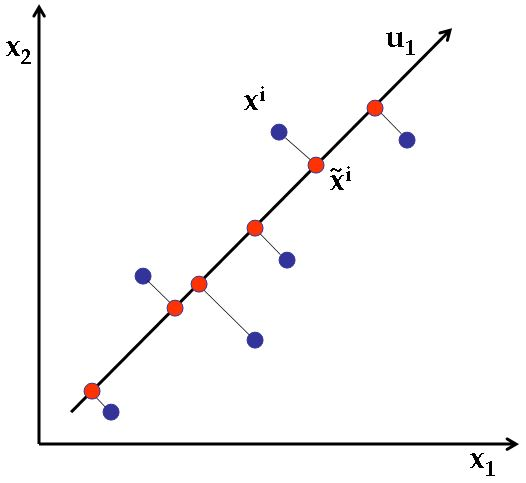
\includegraphics[width=0.38\textwidth]{figures/aBackground/projection}
	\caption{Two-dimensional example of projection of data variables (blue dots) onto PC axes (black). $(u_1)$ indicates the direction of the eigenvector. \cite{PCA2018}}
	\label{projection}
\end{figure}

The algebraic method of calculating the PCs can be done by using Singular Value Decomposition (SVD). The first step is to compute the squared cross product matrix of variances and covariances among every pair of the variables in the data set, where the diagonals are the variances and the off-diagonals are the covariances, as done in the following equation:
%\vspace{-20pt}
\begin{equation}
S = X \textquoteright X
\end{equation}
Where S is the cross product and X is the dataset matrix. When finding the PCs it includes an eigen-analysis of S. The eigenvalues of are solutions to the following equation:
%\verticalspace{1}
\begin{equation}
| S - \lambda I |  = 0
\end{equation}
Where $\lambda$ is the variances of each PC and I is the identity matrix. After solving for $\lambda$ the eigenvectors can be solved through the following equation:
\begin{equation}
det | S - \lambda I | b_{i} = 0
\end{equation}
Where $b_{i}$ is used to calculate the eigenvectors as in:
\begin{eqnarray}
u_{i} = \frac{b_{i}}{\sqrt{b_{i}^{\textquoteright} b_{i}}}
\end{eqnarray}
Where $u_{i}$ is the i number of eigenvectors that contain a contribution to the principal components.
The SVD orders the eigenvalues by size $\lambda_{1} > \lambda_{2} … > \lambda_{i}$. The scores for each PC is equal to the corresponding eigenvalue for that exact axis. The eigenvalues describe how much of the variance is accounted for by the associated PC. Summation of all eigenvalues accounts for the total variance of the data set; this is called the trace. To find how much the each PC accounts for, the eigenvalue of that PC is divided by the total variance: $\%~ of~ total~ variance~ = \frac{\lambda_{i}}{Trace}$. This can be used for deciding how many components are significant and by how much the dataset can be reduced. \cite{Semmlow2004}

\subsection{PCA in images}

The PCA can also be implemented on images, where the dimensionality reduction principle is mostly used for image compression. Here images can be reconstructed using only very few principle components without much information loss. Similarly PCA can be used to de-noise images, as noise would be presented in some of the less saying components, and by removing these, noise would be removed from the image. \\
The PCA can be run on the entire image, but methods introducing local PCA in smaller window of the image, has also been introduced for noise removal. \cite{MuraliMohanBabu2012}   


